\documentclass[12pt]{article}
%\usepackage[letterspace=0]{tgtermes}
% Times New Roman
\usepackage{fontspec}
\setmainfont{Times New Roman}
\usepackage{listings}
\lstset{columns=fullflexible,showstringspaces=false}
% Odstęp między wierszami
\usepackage{setspace}
\singlespacing
\linespread{1}

\usepackage{svg}

% Prefixy rysunków i tabel
\usepackage{caption}
\captionsetup[table]{name=Tab.}
\captionsetup[figure]{name=Rys.}

% Własny rozmiar czcionki
\usepackage{anyfontsize}
\newcommand{\fs}[1]{\fontsize{#1}{#1}\selectfont}

% Inne ustawienia

% Własne komendy
\newcommand{\listsinglespacing}{\setlength{\itemsep}{1pt}\setlength{\parskip}{0pt}\setlength{\parsep}{0pt}}

\usepackage{xcolor,listings}

\usepackage[nosingleletter]{impnattypo}
% Language setting
% Replace `english' with e.g. `spanish' to change the document language
\usepackage[utf8]{inputenc}
\usepackage{polski}
\usepackage[polish]{babel}
\usepackage[linewidth=1pt]{mdframed}
% Set page size and margins
% Replace `letterpaper' with `a4paper' for UK/EU standard size
\usepackage[letterpaper,top=2cm,bottom=2cm,left=2cm,right=2cm,marginparwidth=2cm]{geometry}

% Useful packages
\usepackage{amsmath}
\usepackage{graphicx}
\usepackage[colorlinks=true, allcolors=blue]{hyperref}




\begin{document}
\title{
   
\includegraphics[width=0.4\textwidth]{Images/wsiiz-logo-transparent.png}~\\[1cm]
  \textbf{\fs{16}{Wyższa Szkoła Informatyki i Zarządzania }\\
  \fs{16}{ Kolegium Informatyki Stosowanej, Informatyka}
  }}
  \author{\fs{15}{Rafał Wątroba, w65575}}\vfill   
\date{}

\maketitle
\begin{center}
  \textbf{\emph{\fs{20}{Projekt Bazodanowy dla Szpitala}}} 

    \vfill
    \textbf{\fs{14}{Rzeszów, 06.01.2023  }}
\end{center}
\thispagestyle{empty} % usuwa numerowanie
\newpage

% Zadnie 1 
%\section*{Dane}
\par{
Baza danych obsługująca szpital wraz z obsługą zabiegów. Lekarze będą mogli dodawać przyjęcie pacjenta na wizytę. Wypisywanie skierowania na zabiegi i badania, przepisywanie recept. Pielęgniarki będą miały możliwość dodawania nowego pacjenta, edycje informacji o badaniach, oraz rejestrację na wizytę domową. Pacjenci będą mogli otrzymać informacje o swoich receptach i nadchodzących badaniach i zabiegach. Również będą mieli wgląd do swoich danych z przebiegu choroby, historii poprzednich badań i zabiegów. Spedytorzy będą mieli wgląd w historię wyjazdów karetek, skład załóg w karetkach oraz możliwość dodawania nowego wyjazdu.
}
%%\section*{Raporty:}\\
\begin{enumerate}
\itemsep-5pt
\item Raport z wyjazdu karetki w wybranym dniu,
\item Ilość zaplanowanych wizyt dla lekarza na dany dzień,
\item Ilość przeprowadzonego zabiegu w danym miesiącu,
\item Informacja o ilości osób przyjętych ze złamaniami,
\item Ilość kobiet przyjętych na oddział położniczy,
\item Informacje o historii zabiegów pacjenta,
\item Recepta dla Pacjenta,
\item Historia choroby pacjenta.

\end{enumerate}
Podczas dalszej pracy nad projektem ilość zestawień ulegnie zwiększeniu.
%\section*{Zestawienia:}\\
    \begin{enumerate}
        \itemsep-5pt
\item Zestawienie ilości powodów przyjęć pacjentów na SOR,
\item Zestawienie rocznych wyjazdów karetek podzielone na miesiące,
\item Zestawienie różnych zabiegów na przestrzeni miesiąca,
\item Średnia ilość pacjentów w danych miesiącach,
\item Pracownicy o danym imieniu,
\item Średnia ilość recept,
\item Ilość osób, które zachorowały na grypę w okresie zimowym w przeciągu ostatnich 3 lat.
\end{enumerate}
Podczas dalszej pracy nad projektem ilość zestawień ulegnie zwiększeniu.
\section*{Dane}
\par{
Baza danych obsługująca szpital wraz z obsługą zabiegów. Lekarze będą mogli dodawać przyjęcie pacjenta na wizytę. Wypisywanie skierowania na zabiegi i badania, przepisywanie recept. Pielęgniarki będą miały możliwość dodawania nowego pacjenta, edycje informacji o badaniach, oraz rejestrację na wizytę domową. Pacjenci będą mogli otrzymać informacje o swoich receptach i nadchodzących badaniach i zabiegach. Również będą mieli wgląd do swoich danych z przebiegu choroby, historii poprzednich badań i zabiegów. Spedytorzy będą mieli wgląd w historię wyjazdów karetek, skład załóg w karetkach oraz możliwość dodawania nowego wyjazdu.
}
\section*{Raporty:}\\
\begin{enumerate}
\itemsep-5pt
\item Raport z wyjazdu karetki w wybranym dniu,
\item Ilość zaplanowanych wizyt dla lekarza na dany dzień,
\item Ilość przeprowadzonego zabiegu w danym miesiącu,
\item Informacja o ilości osób przyjętych ze złamaniami,
\item Ilość kobiet przyjętych na oddział położniczy,
\item Informacje o historii zabiegów pacjenta,
\item Recepta dla Pacjenta,
\item Historia choroby pacjenta.

\end{enumerate}
Podczas dalszej pracy nad projektem ilość zestawień ulegnie zwiększeniu.

\section*{Zestawienia:}\\
    \begin{enumerate}
        \itemsep-5pt
\item Zestawienie ilości powodów przyjęć pacjentów na SOR,
\item Zestawienie rocznych wyjazdów karetek podzielone na miesiące,
\item Zestawienie różnych zabiegów na przestrzeni miesiąca,
\item Średnia ilość pacjentów w danych miesiącach,
\item Pracownicy o danym imieniu,
\item Średnia ilość recept,
\item Ilość osób, które zachorowały na grypę w okresie zimowym w przeciągu ostatnich 3 lat.
\end{enumerate}
Podczas dalszej pracy nad projektem ilość zestawień ulegnie zwiększeniu.
\newpage

% Zadnie 2
\section*{\fs{12}Diagram}
\par{
\fs{12}

\begin{figure}[h!]
    \centering
   \scalebox{.35}{ 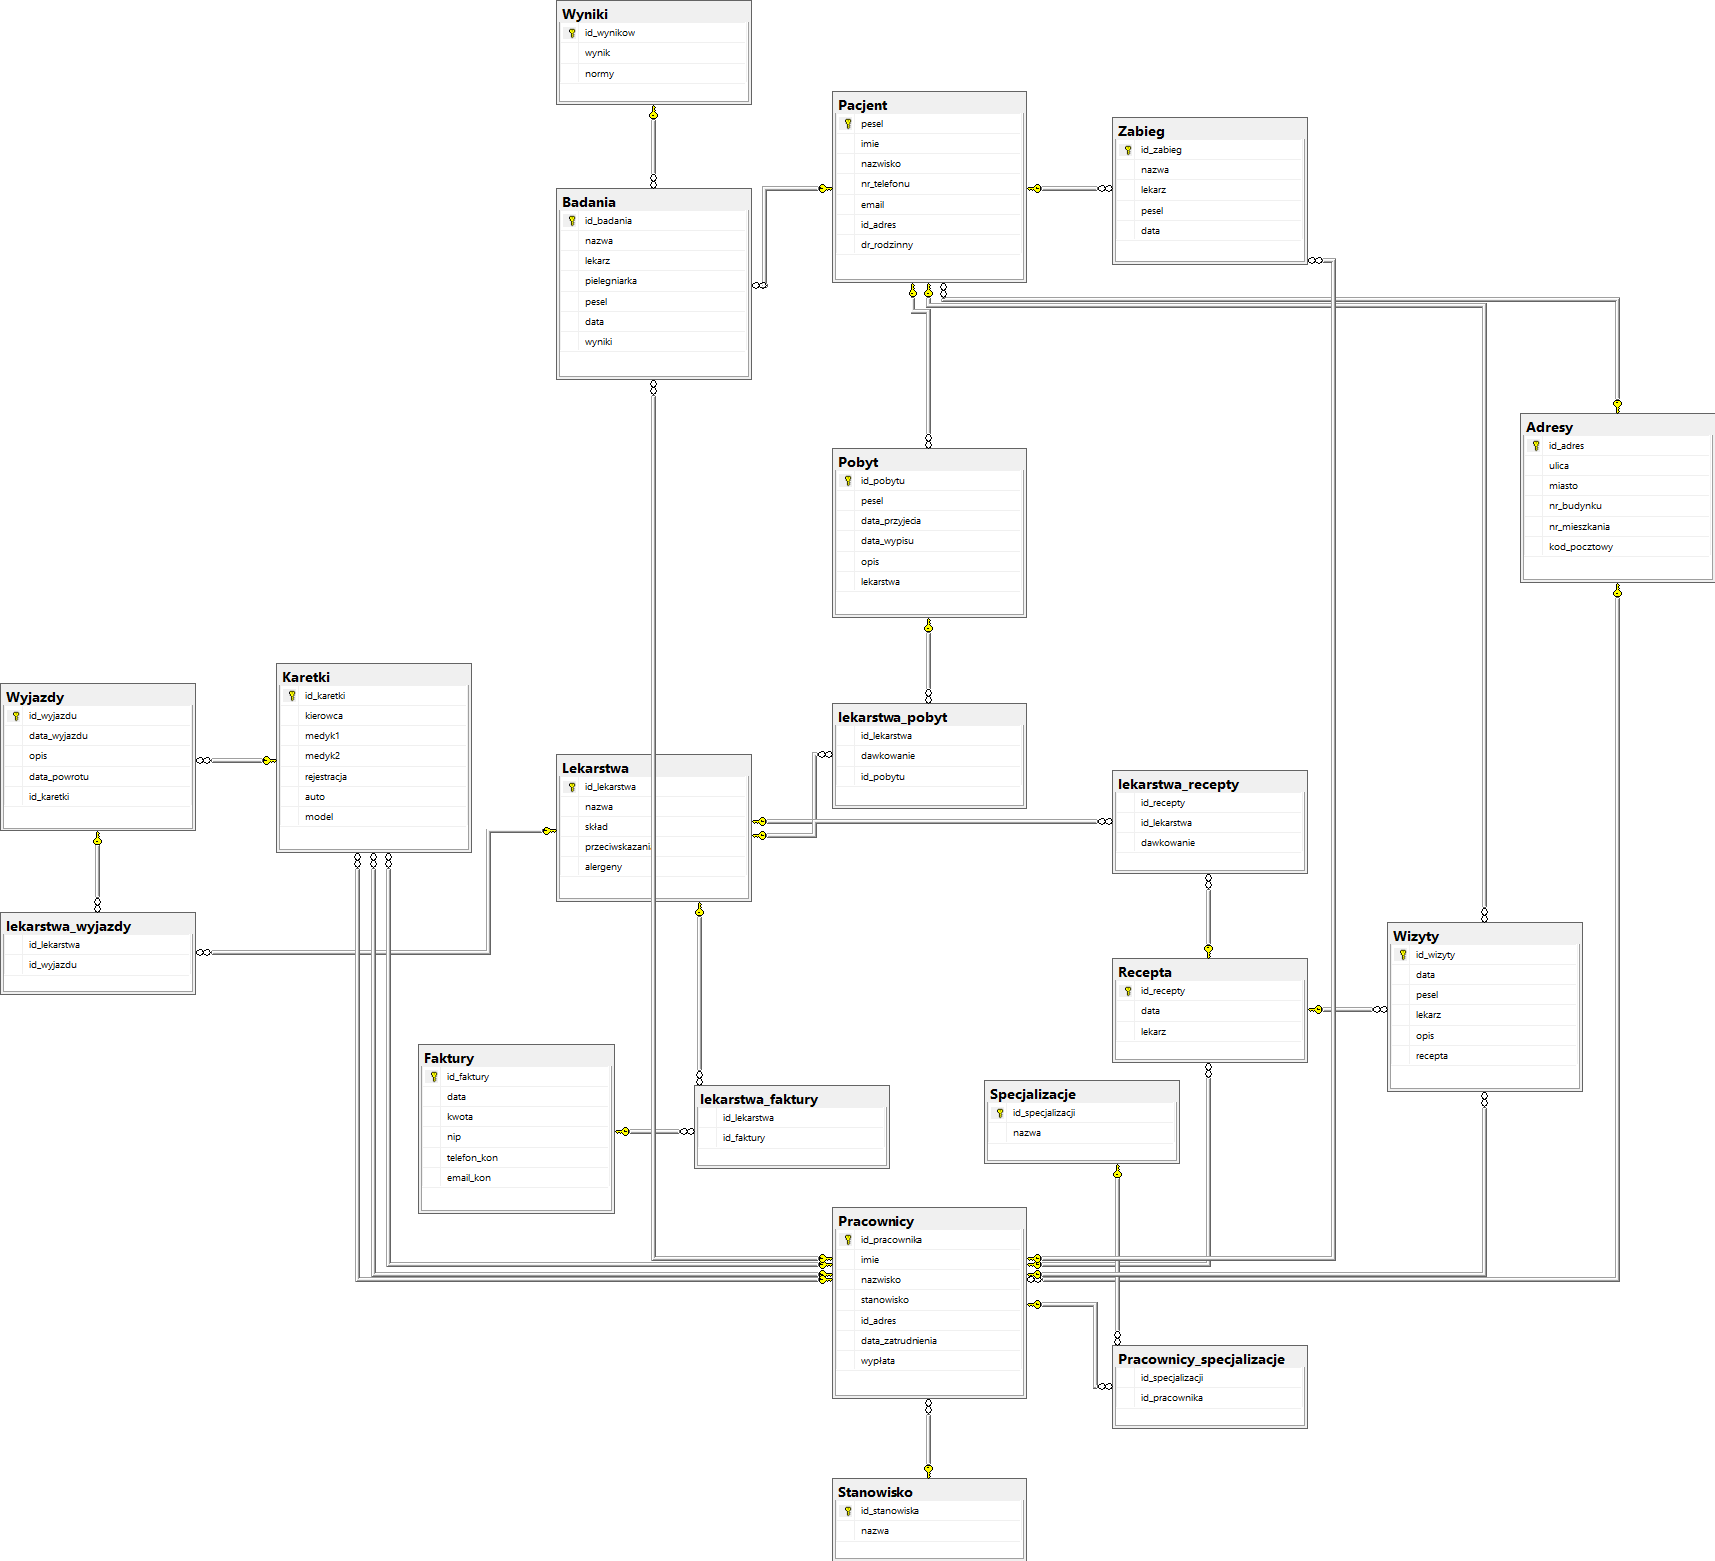
\includegraphics{Images/Zadanie2/Diagram1.png}}
    \caption{Diagram ERD}
    \label{fig:my_label}
\end{figure}
}
\newpage
\section*{\fs{12}Tablica Adresy}
\par{
\fs{12}

\begin{figure}[h!]
    \centering
   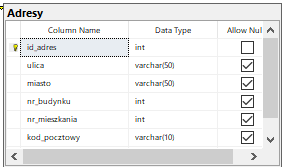
\includegraphics{Images/Zadanie2/Adresy.png}
    \caption{Tablica Adresy}
    \label{fig:my_label}
\end{figure}

\listsinglespacing{
\fs{12}
\begin{lstlisting}[frame=single,language=SQL,]
Select * from adresy

\end{lstlisting}

}

\begin{figure}[h!]
    \centering
   \scalebox{.65}{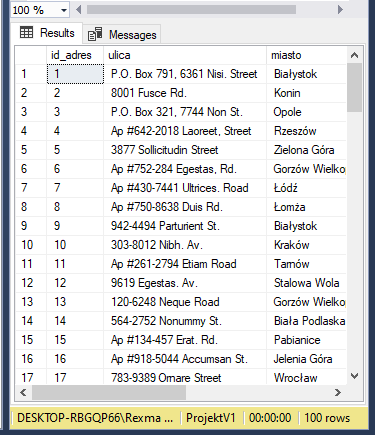
\includegraphics{Images/Zadanie2/Zapelnione/adresy_query.png}}
    \caption{Wynik Zapytania}
    \label{fig:my_label}
\end{figure}
}
\newpage
\section*{\fs{12}Tablica Badania}
\par{
\fs{12}

\begin{figure}[h!]
    \centering
   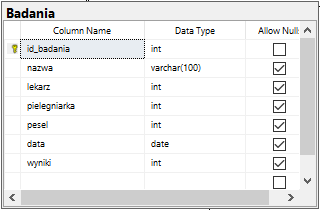
\includegraphics{Images/Zadanie2/Badania.png}
    \caption{Tablica Badania}
    \label{fig:my_label}
\end{figure}


\listsinglespacing{
\fs{12}
\begin{lstlisting}[frame=single,language=SQL,]
Select * from Badania

\end{lstlisting}

\begin{figure}[h!]
    \centering
   \scalebox{.85}{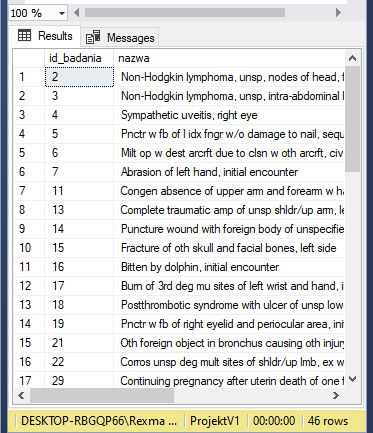
\includegraphics{Images/Zadanie2/Zapelnione/badania_query.png}}
    \caption{Wynik Zapytania}
    \label{fig:my_label}
\end{figure}
}
\newpage
\section*{\fs{12}Tablica Faktury}
\par{
\fs{12}

\begin{figure}[h!]
    \centering
   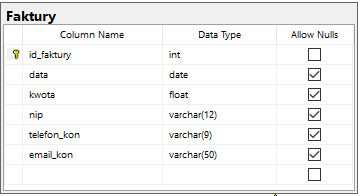
\includegraphics{Images/Zadanie2/Faktury.png}
    \caption{Tablica Faktury}
    \label{fig:my_label}
\end{figure}


\listsinglespacing{
\fs{12}
\begin{lstlisting}[frame=single,language=SQL,]
Select * from Faktury

\end{lstlisting}

\begin{figure}[h!]
    \centering
   \scalebox{.85}{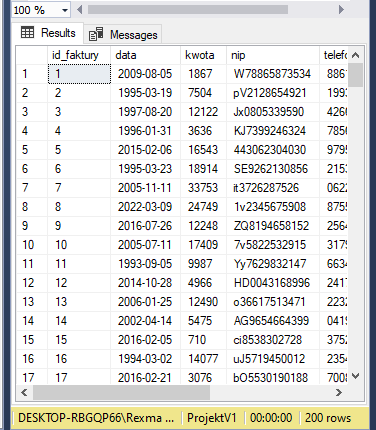
\includegraphics{Images/Zadanie2/Zapelnione/Faktury_query.png}}
    \caption{Wynik Zapytania}
    \label{fig:my_label}
\end{figure}
}
\newpage
\section*{\fs{12}Tablica Karetki}
\par{
\fs{12}

\begin{figure}[h!]
    \centering
   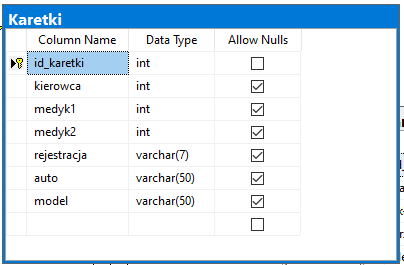
\includegraphics{Images/Zadanie2/Karetki.png}
    \caption{Tablica Karetki}
    \label{fig:my_label}
\end{figure}

\listsinglespacing{
\fs{12}
\begin{lstlisting}[frame=single,language=SQL,]
Select * from Karetki

\end{lstlisting}
\begin{figure}[h!]
    \centering
   \scalebox{.85}{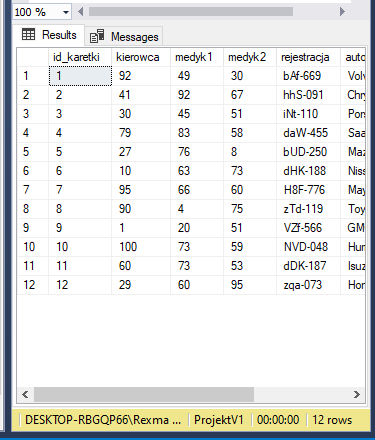
\includegraphics{Images/Zadanie2/Zapelnione/Karetki_query.png}}
    \caption{Wynik Zapytania}
    \label{fig:my_label}
\end{figure}
}
\newpage
\section*{\fs{12}Tablica lekarstwa-faktury}
\par{
\fs{12}

\begin{figure}[h!]
    \centering
   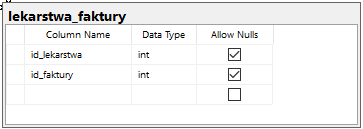
\includegraphics{Images/Zadanie2/lekarstwa_faktury.png}
    \caption{Tablica lekarstwa-faktury}
    \label{fig:my_label}
\end{figure}

\listsinglespacing{
\fs{12}
\begin{lstlisting}[frame=single,language=SQL,]
Select * from lekarstwa-faktury

\end{lstlisting}
\begin{figure}[h!]
    \centering
   \scalebox{.85}{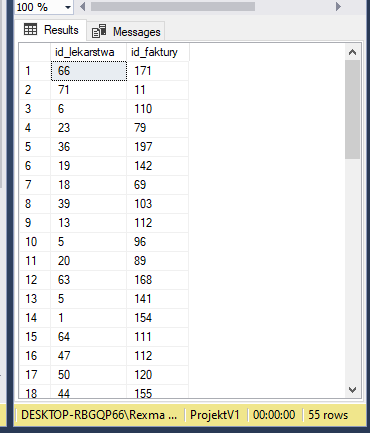
\includegraphics{Images/Zadanie2/Zapelnione/lekarstwa_faktury_query.png}}
    \caption{Wynik Zapytania}
    \label{fig:my_label}
\end{figure}
}
\newpage
\section*{\fs{12}Tablica lekarstwa-pobyt}
\par{
\fs{12}

\begin{figure}[h!]
    \centering
   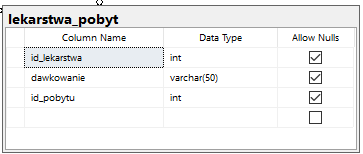
\includegraphics{Images/Zadanie2/lekarstwa_pobyt.png}
    \caption{Tablica lekarstwa-pobyt}
    \label{fig:my_label}
\end{figure}


\listsinglespacing{
\fs{12}
\begin{lstlisting}[frame=single,language=SQL,]
Select * from lekarstwa-pobyt

\end{lstlisting}

\begin{figure}[h!]
    \centering
   \scalebox{.85}{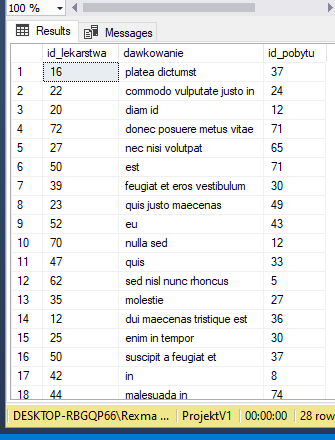
\includegraphics{Images/Zadanie2/Zapelnione/lekarstwa_pobyt_query.png}}
    \caption{Wynik Zapytania}
    \label{fig:my_label}
\end{figure}
}
\newpage
\section*{\fs{12}Tablica lekarstwa-recepty}
\par{
\fs{12}

\begin{figure}[h!]
    \centering
   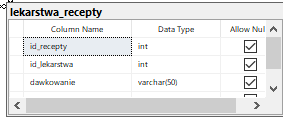
\includegraphics{Images/Zadanie2/lekarstwa_recepty.png}
    \caption{Tablica lekarstwa-recepty}
    \label{fig:my_label}
\end{figure}

\listsinglespacing{
\fs{12}
\begin{lstlisting}[frame=single,language=SQL,]
Select * from lekarstwa-recepty

\end{lstlisting}
\begin{figure}[h!]
    \centering
   \scalebox{.85}{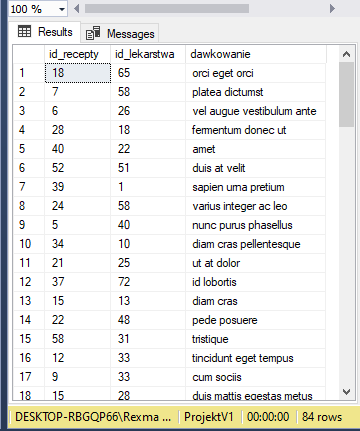
\includegraphics{Images/Zadanie2/Zapelnione/lekarstwa_recepty__query.png}}
    \caption{Wynik Zapytania}
    \label{fig:my_label}
\end{figure}
}
\newpage
\section*{\fs{12}Tablica lekarstwa-recepty}
\par{
\fs{12}

\begin{figure}[h!]
    \centering
   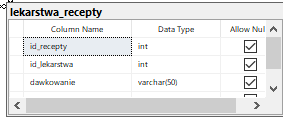
\includegraphics{Images/Zadanie2/lekarstwa_recepty.png}
    \caption{Tablica lekarstwa-recepty}
    \label{fig:my_label}
\end{figure}

\listsinglespacing{
\fs{12}
\begin{lstlisting}[frame=single,language=SQL,]
Select * from lekarstwa-recepty

\end{lstlisting}
\begin{figure}[h!]
    \centering
   \scalebox{.85}{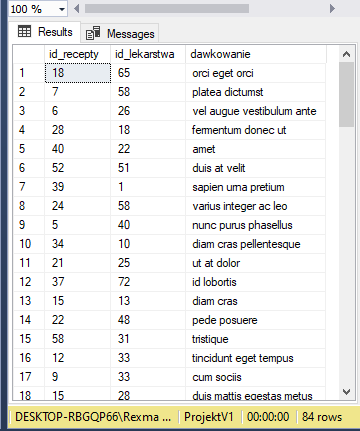
\includegraphics{Images/Zadanie2/Zapelnione/lekarstwa_recepty__query.png}}
    \caption{Wynik Zapytania}
    \label{fig:my_label}
\end{figure}
}
\newpage
\section*{\fs{12}Tablica lekarstwa-wyjazdy}
\par{
\fs{12}

\begin{figure}[h!]
    \centering
   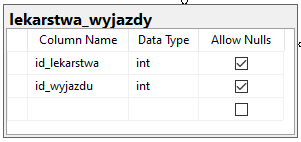
\includegraphics{Images/Zadanie2/lekarstwa_wyjazdy.png}
    \caption{Tablica lekarstwa-wyjazdy}
    \label{fig:my_label}
\end{figure}\listsinglespacing{
\fs{12}
\begin{lstlisting}[frame=single,language=SQL,]
Select * from lekarstwa-wyjazdy

\end{lstlisting}
\begin{figure}[h!]
    \centering
   \scalebox{.85}{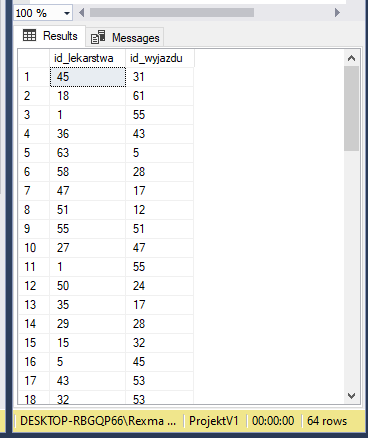
\includegraphics{Images/Zadanie2/Zapelnione/lekarstw_wyjazdy_query.png}}
    \caption{Wynik Zapytania}
    \label{fig:my_label}
\end{figure}
}
\newpage
\section*{\fs{12}Tablica Lekarstwa}
\par{
\fs{12}

\begin{figure}[h!]
    \centering
   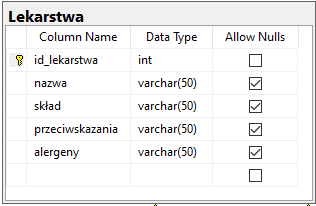
\includegraphics{Images/Zadanie2/Lekarstwa.png}
    \caption{Tablica Lekarstwa}
    \label{fig:my_label}
\end{figure}
\listsinglespacing{
\fs{12}
\begin{lstlisting}[frame=single,language=SQL,]
Select * from Lekarstwa

\end{lstlisting}
\begin{figure}[h!]
    \centering
   \scalebox{.85}{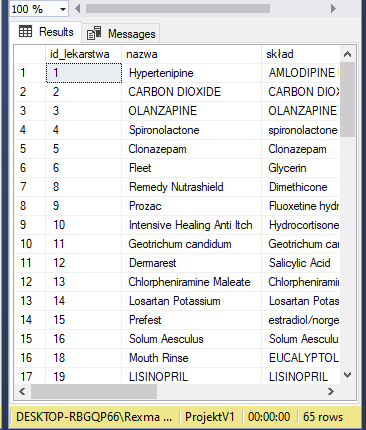
\includegraphics{Images/Zadanie2/Zapelnione/Lekarstwa_query.png}}
    \caption{Wynik Zapytania}
    \label{fig:my_label}
\end{figure}
}
\newpage
\section*{\fs{12}Tablica Pacjent}
\par{
\fs{12}

\begin{figure}[h!]
    \centering
   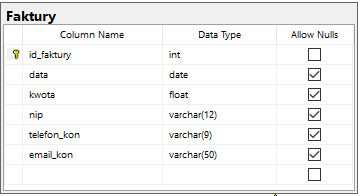
\includegraphics{Images/Zadanie2/Faktury.png}
    \caption{Tablica Pacjent}
    \label{fig:my_label}
\end{figure}
\listsinglespacing{
\fs{12}
\begin{lstlisting}[frame=single,language=SQL,]
Select * from Pacjent

\end{lstlisting}
\begin{figure}[h!]
    \centering
   \scalebox{.85}{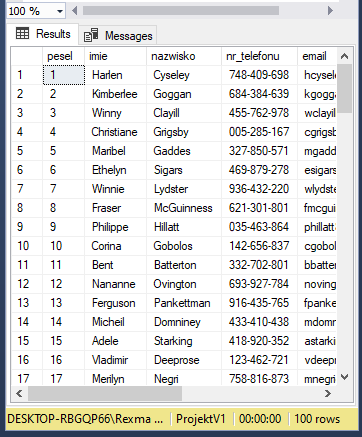
\includegraphics{Images/Zadanie2/Zapelnione/Pacjent_query.png}}
    \caption{Wynik Zapytania}
    \label{fig:my_label}
\end{figure}
}
\newpage
\section*{\fs{12}Tablica Pobyt}
\par{
\fs{12}

\begin{figure}[h!]
    \centering
   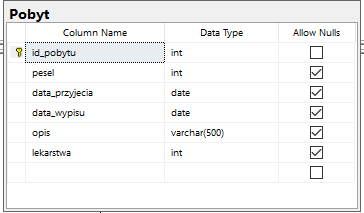
\includegraphics{Images/Zadanie2/Pobyt.png}
    \caption{Tablica Pobyt}
    \label{fig:my_label}
\end{figure}
\listsinglespacing{
\fs{12}
\begin{lstlisting}[frame=single,language=SQL,]
Select * from Pobyt

\end{lstlisting}
\begin{figure}[h!]
    \centering
   \scalebox{.85}{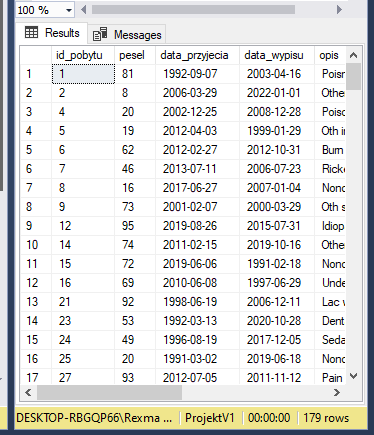
\includegraphics{Images/Zadanie2/Zapelnione/Pobyt_query.png}}
    \caption{Wynik Zapytania}
    \label{fig:my_label}
\end{figure}
}
\newpage
\section*{\fs{12}Tablica pracownicy-specjalizacje}
\par{
\fs{12}

\begin{figure}[h!]
    \centering
   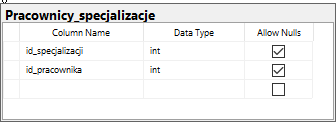
\includegraphics{Images/Zadanie2/Pracownicy_specjalizacje.png}
    \caption{Tablica pracownicy-specjalizacje}
    \label{fig:my_label}
\end{figure}
\listsinglespacing{
\fs{12}
\begin{lstlisting}[frame=single,language=SQL,]
Select * from pracownicy-specjalizacje

\end{lstlisting}
\begin{figure}[h!]
    \centering
   \scalebox{.85}{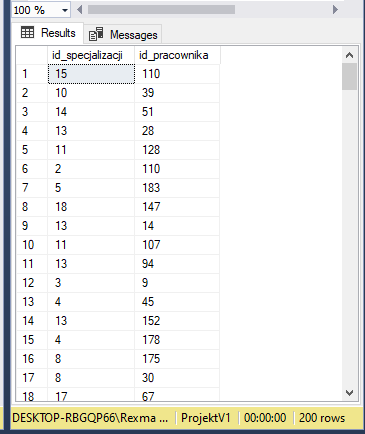
\includegraphics{Images/Zadanie2/Zapelnione/Pracownicy_specjalizacje_query.png}}
    \caption{Wynik Zapytania}
    \label{fig:my_label}
\end{figure}
}
\newpage
\section*{\fs{12}Tablica Pracownicy}
\par{
\fs{12}

\begin{figure}[h!]
    \centering
   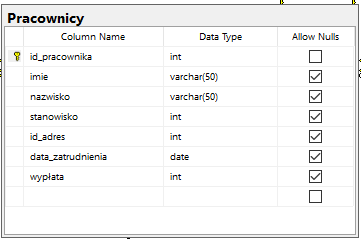
\includegraphics{Images/Zadanie2/Pracownicy.png}
    \caption{Tablica Pracownicy}
    \label{fig:my_label}
\end{figure}
\listsinglespacing{
\fs{12}
\begin{lstlisting}[frame=single,language=SQL,]
Select * from Pracownicy

\end{lstlisting}
\begin{figure}[h!]
    \centering
   \scalebox{.85}{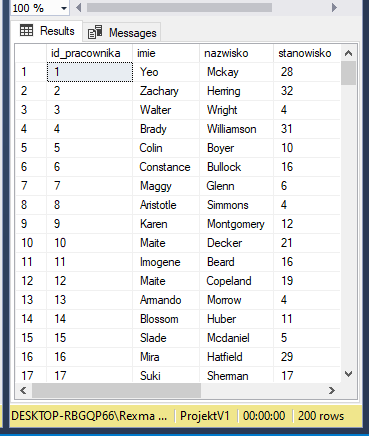
\includegraphics{Images/Zadanie2/Zapelnione/Pracownicy_query.png}}
    \caption{Wynik Zapytania}
    \label{fig:my_label}
\end{figure}
}
\newpage
\section*{\fs{12}Tablica Recepty}
\par{
\fs{12}

\begin{figure}[h!]
    \centering
   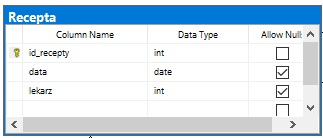
\includegraphics{Images/Zadanie2/Recepta.png}
    \caption{Tablica Recepty}
    \label{fig:my_label}
\end{figure}
\listsinglespacing{
\fs{12}
\begin{lstlisting}[frame=single,language=SQL,]
Select * from Recepty

\end{lstlisting}
\begin{figure}[h!]
    \centering
   \scalebox{.85}{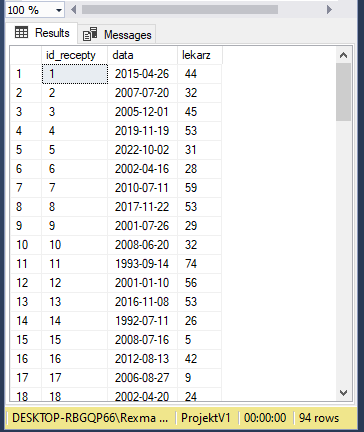
\includegraphics{Images/Zadanie2/Zapelnione/Recepta_query.png}}
    \caption{Wynik Zapytania}
    \label{fig:my_label}
\end{figure}
}
\newpage
\section*{\fs{12}Tablica Specjalizacje}
\par{
\fs{12}

\begin{figure}[h!]
    \centering
   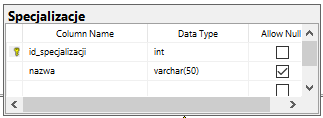
\includegraphics{Images/Zadanie2/Secjalizacje.png}
    \caption{Tablica Specjalizacje}
    \label{fig:my_label}
\end{figure}\listsinglespacing{
\fs{12}
\begin{lstlisting}[frame=single,language=SQL,]
Select * from Specjalizacje

\end{lstlisting}
\begin{figure}[h!]
    \centering
   \scalebox{.85}{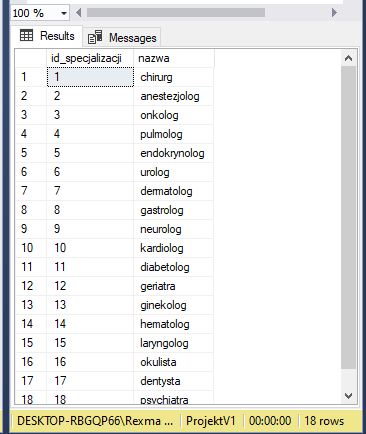
\includegraphics{Images/Zadanie2/Zapelnione/Specjalizacje_query.png}}
    \caption{Wynik Zapytania}
    \label{fig:my_label}
\end{figure}
}
\newpage
\section*{\fs{12}Tablica Stanowisko}
\par{
\fs{12}

\begin{figure}[h!]
    \centering
   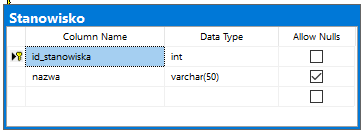
\includegraphics{Images/Zadanie2/Stanowisko.png}
    \caption{Tablica Stanowisko}
    \label{fig:my_label}
\end{figure}\listsinglespacing{
\fs{12}
\begin{lstlisting}[frame=single,language=SQL,]
Select * from  Stanowisko

\end{lstlisting}
\begin{figure}[h!]
    \centering
   \scalebox{.85}{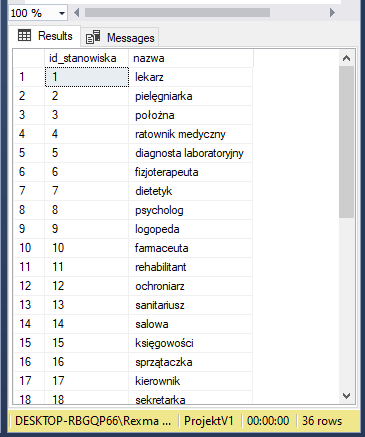
\includegraphics{Images/Zadanie2/Zapelnione/Stanowisko_query.png}}
    \caption{Wynik Zapytania}
    \label{fig:my_label}
\end{figure}
}
\newpage
\section*{\fs{12}Tablica Wizyty}
\par{
\fs{12}

\begin{figure}[h!]
    \centering
   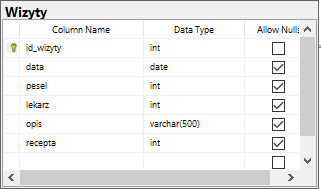
\includegraphics{Images/Zadanie2/Wizyty.png}
    \caption{Tablica Wizyty}
    \label{fig:my_label}
\end{figure}
\listsinglespacing{
\fs{12}
\begin{lstlisting}[frame=single,language=SQL,]
Select * from Wizyty

\end{lstlisting}
\begin{figure}[h!]
    \centering
   \scalebox{.85}{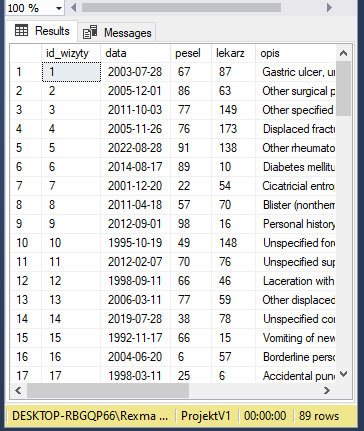
\includegraphics{Images/Zadanie2/Zapelnione/Wizyty_query.png}}
    \caption{Wynik Zapytania}
    \label{fig:my_label}
\end{figure}
}
\newpage
\section*{\fs{12}Tablica Wyjazdy}
\par{
\fs{12}

\begin{figure}[h!]
    \centering
   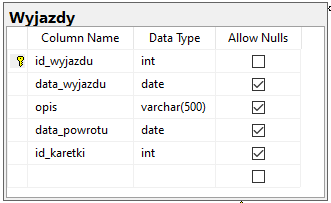
\includegraphics{Images/Zadanie2/Wyjazdy.png}
    \caption{Tablica Wyjazdy}
    \label{fig:my_label}
\end{figure}
\listsinglespacing{
\fs{12}
\begin{lstlisting}[frame=single,language=SQL,]
Select * from Wyjazdy

\end{lstlisting}
\begin{figure}[h!]
    \centering
   \scalebox{.85}{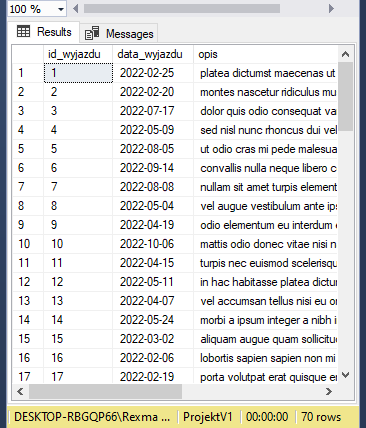
\includegraphics{Images/Zadanie2/Zapelnione/Wyjazdy_query.png}}
    \caption{Wynik Zapytania}
    \label{fig:my_label}
\end{figure}
}
\newpage
\section*{\fs{12}Tablica Wyniki}
\par{
\fs{12}

\begin{figure}[h!]
    \centering
   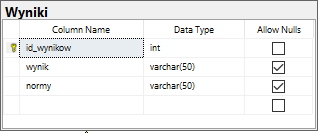
\includegraphics{Images/Zadanie2/Wyniki.png}
    \caption{Tablica Wyniki}
    \label{fig:my_label}
\end{figure}
\listsinglespacing{
\fs{12}
\begin{lstlisting}[frame=single,language=SQL,]
Select * from Wyniki

\end{lstlisting}
\begin{figure}[h!]
    \centering
   \scalebox{.85}{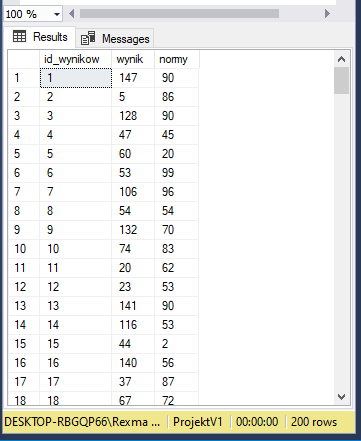
\includegraphics{Images/Zadanie2/Zapelnione/Wyniki_query.png}}
    \caption{Wynik Zapytania}
    \label{fig:my_label}
\end{figure}
}
\newpage
\section*{\fs{12}Tablica Zabiegi}
\par{
\fs{12}

\begin{figure}[h!]
    \centering
   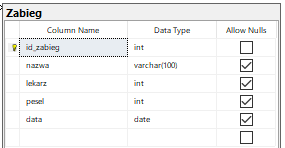
\includegraphics{Images/Zadanie2/Zabieg.png}
    \caption{Tablica Zabieg}
    \label{fig:my_label}
\end{figure}
\listsinglespacing{
\fs{12}
\begin{lstlisting}[frame=single,language=SQL,]
Select * from Zabiegi

\end{lstlisting}
\begin{figure}[h!]
    \centering
   \scalebox{.85}{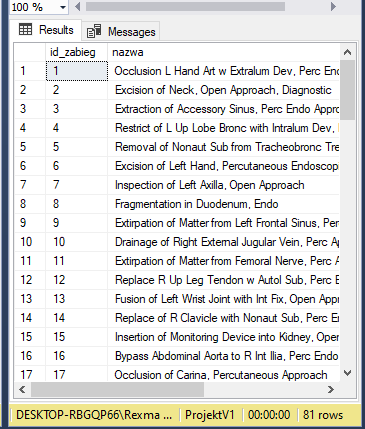
\includegraphics{Images/Zadanie2/Zapelnione/Zabiegi_query.png}}
    \caption{Wynik Zapytania}
    \label{fig:my_label}
\end{figure}
}
% Zadanie 3

\section*{\fs{12}Zapytanie do jednej tablicy}
\subsection*{\fs{12} Data zatrudnienia Trevor Sanford }
\par{
\fs{12}


\listsinglespacing{
\fs{12}
\begin{lstlisting}[frame=single,language=SQL,]
Select data_zatrudnienia as Zatrudniony
from  Pracownicy
where imie='Trevor' and nazwisko='Sanford'

\end{lstlisting}
\begin{figure}[h!]
    \centering
   \scalebox{.85}{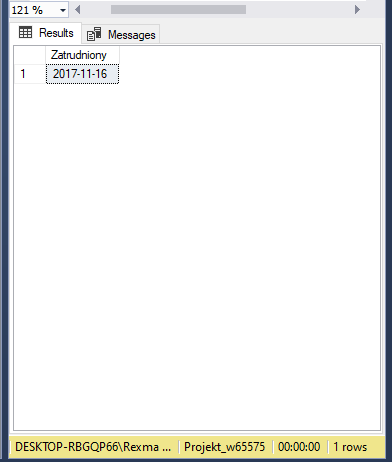
\includegraphics{Images/Zadanie3/P1/Z1a.png}}
    \caption{Wynik Zapytania}
    \label{fig:my_label}
\end{figure}

}
\begin{figure}[h!]
    \centering
   \scalebox{.70}{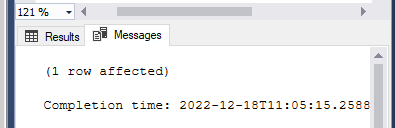
\includegraphics{Images/Zadanie3/P1/Z1b.png}}
    \caption{Wynik Zapytania}
    \label{fig:my_label}
\end{figure}
}
\newpage

\subsection*{\fs{12} Pracownicy zarabiajacy ponad 10000 w kolejnosci alfabetyczne }
\listsinglespacing{
\fs{12}
\begin{lstlisting}[frame=single,language=SQL,]
Select imie,nazwisko
from  Pracownicy
where wypłata>=10000
order by nazwisko

\end{lstlisting}
\begin{figure}[h!]
    \centering
   \scalebox{.85}{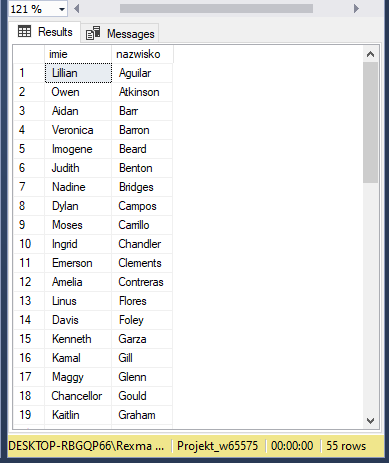
\includegraphics{Images/Zadanie3/P1/Z2a.png}}
    \caption{Wynik Zapytania}
    \label{fig:my_label}
\end{figure}

}

\begin{figure}[h!]
    \centering
   \scalebox{.70}{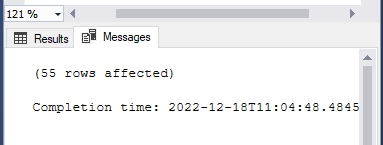
\includegraphics{Images/Zadanie3/P1/Z2b.png}}
    \caption{Wynik Zapytania}
    \label{fig:my_label}
\end{figure}


\newpage
\subsection*{\fs{12} Nr telefonu do  Zorana	Deroche}
\listsinglespacing{
\fs{12}
\begin{lstlisting}[frame=single,language=SQL,]
Select nr_telefonu as Kontakt
from  Pacjent
where imie='Zorana' and nazwisko='Deroche'

\end{lstlisting}
\begin{figure}[h!]
    \centering
   \scalebox{.85}{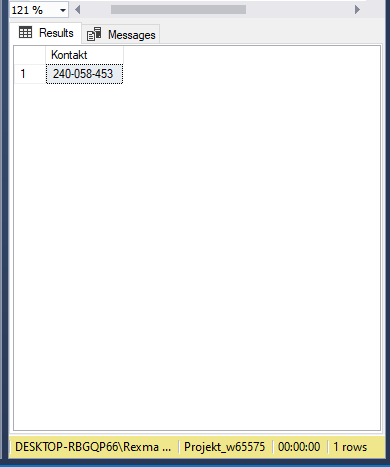
\includegraphics{Images/Zadanie3/P1/Z3a.png}}
    \caption{Wynik Zapytania}
    \label{fig:my_label}
\end{figure}

}
\begin{figure}[h!]
    \centering
   \scalebox{.70}{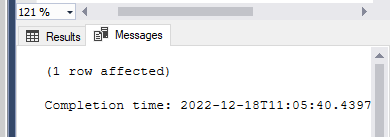
\includegraphics{Images/Zadanie3/P1/Z3b.png}}
    \caption{Wynik Zapytania}
    \label{fig:my_label}
\end{figure}

\newpage

\subsection*{\fs{12} Wypisanie zarobków}
\listsinglespacing{
\fs{12}
\begin{lstlisting}[frame=single,language=SQL,]
Select imie,nazwisko, 
CASE
	When Wypłata<5000 THEN 'Zarabia mało'
	WHEN Wypłata>5000 THEN 'Zarabia średnio'
	WHEN Wypłata>10000 THEN 'Zarabia dużo'
END
as [Ile zarabia]
from Pracownicy

\end{lstlisting}
}
\begin{figure}[h!]
    \centering
   \scalebox{.85}{\includegraphics{Images/Zadanie3/P1/Z4a.png}}
    \caption{Wynik Zapytania}
    \label{fig:my_label}
\end{figure}
\begin{figure}[h!]
    \centering
   \scalebox{.70}{\includegraphics{Images/Zadanie3/P1/Z4b.png}}
    \caption{Wynik Zapytania}
    \label{fig:my_label}
\end{figure}\newpage

\subsection*{\fs{12} Wygnerowanie emailów dla pracowników}
\listsinglespacing{
\fs{12}
\begin{lstlisting}[frame=single,language=SQL,]
Select imie,nazwisko,
CONCAT(lower(imie),'-',LOWER(nazwisko),'@hospital.com') as Email 
from Pracownicy

\end{lstlisting}
}
\begin{figure}[h!]
    \centering
   \scalebox{.85}{\includegraphics{Images/Zadanie3/P1/Z5a.png}}
    \caption{Wynik Zapytania}
    \label{fig:my_label}
\end{figure}
\begin{figure}[h!]
    \centering
   \scalebox{.70}{\includegraphics{Images/Zadanie3/P1/Z5b.png}}
    \caption{Wynik Zapytania}
    \label{fig:my_label}
\end{figure}\newpage

\section*{\fs{12}Zapytanie z użyciem Join}
\par{
\fs{12}

\subsection*{\fs{12} Raport z wyjazdu karetki w wybranym dniu.}
\listsinglespacing{
\fs{12}
\begin{lstlisting}[frame=single,language=SQL,]
Select * 
from Wyjazdy 
inner join Karetki on Karetki.id_karetki=Wyjazdy.id_karetki
Where Wyjazdy.data_wyjazdu='2022-02-25';

\end{lstlisting}
\begin{figure}[h!]
    \centering
   \scalebox{.85}{\includegraphics{Images/Zadanie3/P2/Z6a.png}}
    \caption{Wynik Zapytania}
    \label{fig:my_label}
\end{figure}

}
\begin{figure}[h!]
    \centering
   \scalebox{.60}{\includegraphics{Images/Zadanie3/P2/Z6b.png}}
    \caption{Wynik Zapytania}
    \label{fig:my_label}
\end{figure}
\newpage
\subsection*{\fs{12} Ilość zaplanowanych wizyt dla lekarza na dany dzień,}


\listsinglespacing{
\fs{12}
\begin{lstlisting}[frame=single,language=SQL,]
Select * 
from Wizyty inner join Pracownicy on Pracownicy.id_pracownika=Wizyty.lekarz
where Wizyty.data='2001-12-20';

\end{lstlisting}
\begin{figure}[h!]
    \centering
   \scalebox{.85}{\includegraphics{Images/Zadanie3/P2/Z7a.png}}
    \caption{Wynik Zapytania}
    \label{fig:my_label}
\end{figure}

}
\begin{figure}[h!]
    \centering
   \scalebox{.60}{\includegraphics{Images/Zadanie3/P2/Z7b.png}}
    \caption{Wynik Zapytania}
    \label{fig:my_label}
\end{figure}
\newpage
\clearpage
\subsection*{\fs{12} Recepta dla Pacjenta }
\listsinglespacing{
\fs{12}
\begin{lstlisting}[frame=single,language=SQL,]
Create View Pacjent_Recepta as 
Select concat(P.imie,' ',P.nazwisko) as Pacjent , R.data,concat(PR.imie,' ',PR.nazwisko) as Lekarz,
LR.dawkowanie,L.nazwa,L.przeciwskazania,L.skład
from Pacjent as P
inner join Wizyty as W
on P.pesel=W.pesel 
inner join Recepta as R
on W.recepta=R.id_recepty
inner join Pracownicy as PR
on PR.id_pracownika=R.lekarz
inner join lekarstwa_recepty as LR
on LR.id_recepty=R.id_recepty
inner join Lekarstwa as L
on L.id_lekarstwa=LR.id_lekarstwa

Select * from [Pacjent_Recepta]
where YEAR(data) between 2000 and 2010

\end{lstlisting}
\begin{figure}[h!]
    \centering
   \scalebox{.85}{\includegraphics{Images/Zadanie3/P2/Z8a.png}}
    \caption{Wynik Zapytania}
    \label{fig:my_label}
\end{figure}

}

\begin{figure}[h!]
    \centering
   \scalebox{.70}{\includegraphics{Images/Zadanie3/P2/Z8b.png}}
    \caption{Wynik Zapytania}
    \label{fig:my_label}
\end{figure}
\newpage
\clearpage
\subsection*{\fs{12} Numery,Opisy wyjazdów i leki użyte podczas interwencji }
\listsinglespacing{
\fs{12}
\begin{lstlisting}[frame=single,language=SQL,]

Select W.id_wyjazdu,W.data_wyjazdu, W.opis, L.nazwa
from Lekarstwa as L
inner join lekarstwa_wyjazdy as LW
on LW.id_lekarstwa=L.id_lekarstwa
inner join Wyjazdy as W
on W.id_wyjazdu=LW.id_wyjazdu


\end{lstlisting}
\begin{figure}[h!]
    \centering
   \scalebox{.85}{\includegraphics{Images/Zadanie3/P2/Z9a.png}}
    \caption{Wynik Zapytania}
    \label{fig:my_label}
\end{figure}

}

\begin{figure}[h!]
    \centering
   \scalebox{.70}{\includegraphics{Images/Zadanie3/P2/Z9b.png}}
    \caption{Wynik Zapytania}
    \label{fig:my_label}
\end{figure}
\newpage
\clearpage

\subsection*{\fs{12} Badania których wyniki są powyżej normy      }
\listsinglespacing{
\fs{12}
\begin{lstlisting}[frame=single,language=SQL,]
Select Nazwa, Wyniki.wynik,Wyniki.normy
from Badania
inner join Wyniki
on Wyniki.id_wynikow=Badania.wyniki
where wynik>normy

\end{lstlisting}
\begin{figure}[h!]
    \centering
   \scalebox{.85}{\includegraphics{Images/Zadanie3/P2/Z10a.png}}
    \caption{Wynik Zapytania}
    \label{fig:my_label}
\end{figure}

}

\begin{figure}[h!]
    \centering
   \scalebox{.70}{\includegraphics{Images/Zadanie3/P2/Z10b.png}}
    \caption{Wynik Zapytania}
    \label{fig:my_label}
\end{figure}
\newpage
\clearpage
\section*{\fs{12}Zapytanie z użyciem LEFT Join}
\par{
\fs{12}
\subsection*{\fs{12} Ilość kobiet przyjętych na oddział położniczy}

\listsinglespacing{
\fs{12}
\begin{lstlisting}[frame=single,language=SQL,]
Select count(*) as "Ilość kobiet" from Pobyt 
inner join 
(Select id_oddziału,nazwa from Oddział where id_oddziału=13) as O 
ON O.id_oddziału=Pobyt.oddział
left join lekarstwa_pobyt as LP on LP.id_lekarstwa=Pobyt.lekarstwa
left join Pacjent as P on P.pesel=Pobyt.pesel

\end{lstlisting}
\begin{figure}[h!]
    \centering
   \scalebox{.85}{\includegraphics{Images/Zadanie3/P3/Z11a.png}}
    \caption{Wynik Zapytania}
    \label{fig:my_label}
\end{figure}
}
}
\begin{figure}[h!]
    \centering
   \scalebox{.60}{\includegraphics{Images/Zadanie3/P3/Z11b.png}}
    \caption{Wynik Zapytania}
    \label{fig:my_label}
\end{figure}

\newpage
\clearpage

\subsection*{\fs{12} Ilość badań przerowadzonych przez lekarza Owena Gregorego }

\listsinglespacing{
\fs{12}
\begin{lstlisting}[frame=single,language=SQL,]
Select nazwa from Badania
left join Pracownicy
on Pracownicy.id_pracownika=Badania.lekarz
where lekarz ='88'

\end{lstlisting}
\begin{figure}[h!]
    \centering
   \scalebox{.85}{\includegraphics{Images/Zadanie3/P3/Z12a.png}}
    \caption{Wynik Zapytania}
    \label{fig:my_label}
\end{figure}
}
\begin{figure}[h!]
    \centering
   \scalebox{.85}{\includegraphics{Images/Zadanie3/P3/Z12b.png}}
    \caption{Wynik Zapytania}
    \label{fig:my_label}
\end{figure}
\newpage
\subsection*{\fs{12} Pacjenci i ich adresy }

\listsinglespacing{
\fs{12}
\begin{lstlisting}[frame=single,language=SQL,]
Select CONCAT(Imie,' ',nazwisko) as Pacjent, 
CONCAT(miasto, ' ',ulica, ' ' , nr_budynku , ' ',nr_mieszkania) 
as Adres  from Pacjent 
left join Adresy
on Adresy.id_adres=Pacjent.id_adres

\end{lstlisting}
\begin{figure}[h!]
    \centering
   \scalebox{.85}{\includegraphics{Images/Zadanie3/P3/Z13a.png}}
    \caption{Wynik Zapytania}
    \label{fig:my_label}
\end{figure}
}
\begin{figure}[h!]
    \centering
   \scalebox{.60}{\includegraphics{Images/Zadanie3/P3/Z13b.png}}
    \caption{Wynik Zapytania}
    \label{fig:my_label}
\end{figure}
\newpage
\subsection*{\fs{12} Ilosc osób na danych stanowiskach }


\listsinglespacing{
\fs{12}
\begin{lstlisting}[frame=single,language=SQL,]
Select COUNT(*) as [ilosc],S.nazwa  from Pracownicy
left join Stanowisko as S
on Pracownicy.stanowisko=S.id_stanowiska
group by S.nazwa
having count(stanowisko)>=1
order by [ilosc]

\end{lstlisting}
\begin{figure}[h!]
    \centering
   \scalebox{.85}{\includegraphics{Images/Zadanie3/P3/Z14a.png}}
    \caption{Wynik Zapytania}
    \label{fig:my_label}
\end{figure}
}
\begin{figure}[h!]
    \centering
   \scalebox{.60}{\includegraphics{Images/Zadanie3/P3/Z14b.png}}
    \caption{Wynik Zapytania}
    \label{fig:my_label}
\end{figure}\newpage

\newpage
\subsection*{\fs{12} Wizyty }


\listsinglespacing{
\fs{12}
\begin{lstlisting}[frame=single,language=SQL,]
Select W.data,W.opis,
CONCAT(W.pesel,' ',Pa.imie,' ',Pa.nazwisko) as Pacjent,
W.recepta,CONCAT(P.imie,' ',P.nazwisko) as Lekarz
from Wizyty as W
left join Recepta as R
on R.id_recepty=W.recepta
left join Pracownicy as P
on P.id_pracownika=R.id_recepty
left join Pacjent as Pa
on Pa.pesel=W.pesel
order by data

\end{lstlisting}
\begin{figure}[h!]
    \centering
   \scalebox{.85}{\includegraphics{Images/Zadanie3/P3/Z15a.png}}
    \caption{Wynik Zapytania}
    \label{fig:my_label}
\end{figure}
}
\begin{figure}[h!]
    \centering
   \scalebox{.60}{\includegraphics{Images/Zadanie3/P3/Z15b.png}}
    \caption{Wynik Zapytania}
    \label{fig:my_label}
\end{figure}\newpage

\section*{\fs{12}Zapytanie z podzapytaniem w Select}
\par{
\fs{12}
\subsection*{\fs{12} Osoba z największą ilością pobytów w szpitalu}


\listsinglespacing{
\fs{12}
\begin{lstlisting}[frame=single,language=SQL,]
Select TOP 1  imie,nazwisko,
(select COUNT(*) from Pobyt where Pacjent.pesel=Pobyt.pesel) as [Ilość Pobytów w Szpitalu]
from Pacjent 
order by [Ilość Pobytów w Szpitalu] Desc

\end{lstlisting}
\begin{figure}[h!]
    \centering
   \scalebox{.85}{\includegraphics{Images/Zadanie3/P4/Z16a.png}}
    \caption{Wynik Zapytania}
    \label{fig:my_label}
\end{figure}
}
\begin{figure}[h!]
    \centering
   \scalebox{.60}{\includegraphics{Images/Zadanie3/P4/Z16b.png}}
    \caption{Wynik Zapytania}
    \label{fig:my_label}
\end{figure}
\newpage
\subsection*{\fs{12} Imie i Nazwisko pacjeta i nazwa oddziału na jaki został ostatnio przyjęty}

\listsinglespacing{
\fs{12}
\begin{lstlisting}[frame=single,language=SQL,]
Select Imie, nazwisko , 
(Select Top 1  O.Nazwa 
from Pobyt as P inner join 
Oddział as O 
on P.oddział=O.id_oddziału 
where Pacjent.pesel=P.pesel
order by data_przyjecia desc 
)
from Pacjent

\end{lstlisting}
\begin{figure}[h!]
    \centering
   \scalebox{.85}{\includegraphics{Images/Zadanie3/P4/Z17a.png}}
    \caption{Wynik Zapytania}
    \label{fig:my_label}
\end{figure}
}

\begin{figure}[h!]
    \centering
   \scalebox{.60}{\includegraphics{Images/Zadanie3/P4/Z17b.png}}
    \caption{Wynik Zapytania}
    \label{fig:my_label}
\end{figure}
\newpage
\clearpage
\subsection*{\fs{12} Specjalizacje pracowników}
\listsinglespacing{
\fs{12}
\begin{lstlisting}[frame=single,language=SQL,]
Select Imie, Nazwisko, (Select top 1 nazwa from Pracownicy_specjalizacje
inner join Specjalizacje on 
Pracownicy_specjalizacje.id_specjalizacji=Specjalizacje.id_specjalizacji 
where Pracownicy.id_pracownika=Pracownicy_specjalizacje.[id_pracownika])
From Pracownicy

-- wersja z wykorzystaniem with

with spec as (
Select  nazwa,Pracownicy.id_pracownika as idp
from Pracownicy_specjalizacje 
inner join Specjalizacje 
on Pracownicy_specjalizacje.id_specjalizacji=Specjalizacje.id_specjalizacji 
inner join Pracownicy
on Pracownicy.id_pracownika=Pracownicy_specjalizacje.id_pracownika
where Pracownicy.id_pracownika=Pracownicy_specjalizacje.[id_pracownika]
)
Select  imie ,nazwisko,spec.nazwa
from Pracownicy
inner join spec
on spec.idp=Pracownicy.id_pracownika
where spec.nazwa is not null 

\end{lstlisting}
\begin{figure}[h!]
    \centering
   \scalebox{.85}{\includegraphics{Images/Zadanie3/P4/Z18a.png}}
    \caption{Wynik Zapytania}
    \label{fig:my_label}
\end{figure}
}
\begin{figure}[h!]
    \centering
   \scalebox{.60}{\includegraphics{Images/Zadanie3/P4/Z18b.png}}
    \caption{Wynik Zapytania}
    \label{fig:my_label}
\end{figure}
\newpage
\section*{\fs{12}Zapytanie z podzapytaniem w From}
\par{
\fs{12}
\subsection*{\fs{12} Średnia ilość wizyt w ciągu roku}

\listsinglespacing{
\fs{12}
\begin{lstlisting}[frame=single,language=SQL,]
Select WW.ROK,AVG(WW.Ilosc) as [Średnia Roczna]
from (
		Select MONTH(W.data) as Ilosc,YEAR(W.data)  as Rok
		from Wizyty as W
		group by YEAR(W.data), MONTH(W.data)
		)
		as WW
group by WW.Rok

\end{lstlisting}
\begin{figure}[h!]
    \centering
   \scalebox{.85}{\includegraphics{Images/Zadanie3/P5/Z21a.png}}
    \caption{Wynik Zapytania}
    \label{fig:my_label}
\end{figure}
\begin{figure}[h!]
    \centering
   \scalebox{.60}{\includegraphics{Images/Zadanie3/P5/Z21b.png}}
    \caption{Wynik Zapytania}
    \label{fig:my_label}
\end{figure}
}
\newpage
\clearpage

\subsection*{\fs{12} Ilość wyjazdów na przestrzeni lat}

\listsinglespacing{
\fs{12}
\begin{lstlisting}[frame=single,language=SQL,]
Select Count(W.Miesiac) as Wyjazdy, W.Rok
From (
		Select Month(data_wyjazdu) as Miesiac,YEAR(data_wyjazdu) as Rok
		from Wyjazdy
		) as W
Group by W.Rok
\end{lstlisting}
\begin{figure}[h!]
    \centering
   \scalebox{.85}{\includegraphics{Images/Zadanie3/P5/Z22a.png}}
    \caption{Wynik Zapytania}
    \label{fig:my_label}
\end{figure}
\begin{figure}[h!]
    \centering
   \scalebox{.60}{\includegraphics{Images/Zadanie3/P5/Z22b.png}}
    \caption{Wynik Zapytania}
    \label{fig:my_label}
\end{figure}
}
\newpage
\clearpage
\subsection*{\fs{12}Ilość wizyt w poszczególnych miesiącach w roku 2004 }


\listsinglespacing{
\fs{12}
\begin{lstlisting}[frame=single,language=SQL,]
Select Count(W.Dzien) as Ilosc, DATENAME( MONTH, DATEADD( MONTH, W.Miesiac, -1)) 
as Miesiac
From (
		Select Day(data) as Dzien,Month(data) as Miesiac,YEAR(data) as Rok
		from Wizyty 
		where YEAR(data)=2004
		) as W
Group by W.Miesiac

\end{lstlisting}
\begin{figure}[h!]
    \centering
   \scalebox{.85}{\includegraphics{Images/Zadanie3/P5/Z23a.png}}
    \caption{Wynik Zapytania}
    \label{fig:my_label}
\end{figure}

}

\begin{figure}[h!]
    \centering
   \scalebox{.60}{\includegraphics{Images/Zadanie3/P5/Z23b.png}}
    \caption{Wynik Zapytania}
    \label{fig:my_label}
\end{figure}



\newpage
\section*{\fs{12}Zapytanie z podzapytaniem w Where}
\par{
\fs{12}
\subsection*{\fs{12} Imię, nazwisko i wypłatę najlepiej zarabiającego pracownika specjalizującego się w specjalizacji o ID 3.}

\listsinglespacing{
\fs{12}
\begin{lstlisting}[frame=single,language=SQL,]
SELECT imie, nazwisko, wypłata
FROM Pracownicy
WHERE id_pracownika IN 
(SELECT id_pracownika 
FROM Pracownicy_specjalizacje 
WHERE id_specjalizacji = 3)
AND wypłata = (SELECT MAX(wypłata) 
FROM Pracownicy WHERE
id_pracownika IN
(SELECT id_pracownika FROM Pracownicy_specjalizacje WHERE id_specjalizacji = 3))

\end{lstlisting}
\begin{figure}[h!]
    \centering
   \scalebox{.85}{\includegraphics{Images/Zadanie3/P6/Z26a.png}}
    \caption{Wynik Zapytania}
    \label{fig:my_label}
\end{figure}
}
}
\begin{figure}[h!]
    \centering
   \scalebox{.50}{\includegraphics{Images/Zadanie3/P6/Z26b.png}}
    \caption{Wynik Zapytania}
    \label{fig:my_label}
\end{figure}
\newpage
\clearpage
\subsection*{\fs{12} Daty badań przeprowadzonych przez lekarzy z starzem pracy  większym niż 10 lat, posortowane według daty}


\listsinglespacing{
\fs{12}
\begin{lstlisting}[frame=single,language=SQL,]
SELECT convert(varchar, data, 107) AS data
FROM Badania 
WHERE lekarz IN (SELECT P.id_pracownika FROM Pracownicy AS P
WHERE DATEDIFF(year,P.data_zatrudnienia,GETDATE())>10)
order by year(data)
\end{lstlisting}
\begin{figure}[h!]
    \centering
   \scalebox{.85}{\includegraphics{Images/Zadanie3/P6/Z27a.png}}
    \caption{Wynik Zapytania}
    \label{fig:my_label}
\end{figure}
}
\begin{figure}[h!]
    \centering
   \scalebox{.50}{\includegraphics{Images/Zadanie3/P6/Z27b.png}}
    \caption{Wynik Zapytania}
    \label{fig:my_label}
\end{figure}

\newpage
\clearpage
\subsection*{\fs{12} Pacjenci  z Bydgoszczy}


\listsinglespacing{
\fs{12}
\begin{lstlisting}[frame=single,language=SQL,]
Select * 
from Pacjent
Where id_adres IN (Select id_adres from Adresy where miasto='Bydgoszcz')
\end{lstlisting}
\begin{figure}[h!]
    \centering
   \scalebox{.85}{\includegraphics{Images/Zadanie3/P6/Z28a.png}}
    \caption{Wynik Zapytania}
    \label{fig:my_label}
\end{figure}
}
\begin{figure}[h!]
    \centering
   \scalebox{.60}{\includegraphics{Images/Zadanie3/P6/Z28b.png}}
    \caption{Wynik Zapytania}
    \label{fig:my_label}
\end{figure}


\newpage
\end{document}